\chapter{The Lifshitz critical point: methods and results}

As we have seen, the Wetterich equation governs the flow of the scale-dependent effective action $\Gamma_t$. Solving directly this differential equation to find $\Gamma_t$, though in theory possible, is in practice very difficult. Indeed the $\Gamma_t$ depends on the (background) field $\phi$, a function of the momentum. Determining completely $\Gamma_t$ requires knowing its value for all functions $\phi$. 

So, instead of solving directly the Wetterich equation, we start from a reasonable functional form for $\Gamma_t$ with unknown coefficients, we plug it in the Wetterich equation to get flow equations for this coefficients, and we solve these equations.

If we assume that it is analytic in the potential, the effective action can be written as the infinite sum
\begin{equation}
\Gamma_t[\phi] = \int_{x} \left( m_0 (\partial \phi(x))^2 + m_1 (\partial \phi(x)^2)^2 + ... + n_0 (\partial^2 \phi(x))^2 + ... + l_0 \phi(x)^2 + l_1 \phi(x)^3 +... \right)
\end{equation}

This expression can be further simplified if the system under study has some invariance properties. The simplest model having such an invariance is the Ising one, whose microscopic Hamiltonian is invariant under the action of the $\mathds{Z}_2$ symmetry group. If we chose a regulator that preserves this symmetry, it is clear that the effective action $\Gamma_t$ must also be invariant under $\mathds{Z}_2$. The most general expression for $\Gamma_t$ that preserves this symmetry is
\begin{equation}
\label{eq:ising_anzatz}
\Gamma_t^{\text{Ising}}[\phi] = \int_{x} \sum_{i,j \in \mathds{N}} Z_{t,ij} (\partial \phi(x))^{2i} \phi(x)^{2 j}
\end{equation}
The strategy is now simple:
\begin{itemize}
\item Compute $\Gamma_t^{(2)}(x,y)$ from \eqref{eq:ising_anzatz}
\item Plug the result in the right hand side of the Wetterich equation
\item Deduce the flow equation for $Z_{t,ij}$: $\p{t} Z_{t,ij} = F_{i,j}\left( {Z_{t,kl}} \right)$
\end{itemize}
Following this procedure we went from a functional differential equation to a set of simple differential equations. Solving this set of flow equations gives us a complete knowledge of the model. In particular solving the fixed point equations $0 = F_{i,j}\left( {Z^*_{kl}} \right)$ will give us access to the critical properties of the Ising model: critical exponents, critical potential,... Note that for the moment no approximations have been made!

In practice however we know that the lowest degree terms in $\partial \phi$ and $\phi$ will have the most significant contribution to the flow. Therefore we can make the approximation of cutting the development at some order. This has the great practical advantage of reducing the number of flow equations to solve to a finite number. Note that other approximation schemes are possible (development in powers of the field, BMW scheme...). We will not talk about these.

\section{An Anzatz for the Lifshitz scale-dependant effective action}
We recall that the Lifshitz microscopic Hamiltonian is

\begin{equation}
H[\phi] = \int_x \left( \frac{1}{2}(\p{\perp} \phi)^2 + \frac{\rho_0}{2}(\p{\sslash} \phi)^2 + \frac{\sigma_0}{2} (\p{\sslash}^2 \phi)^2 + U(\rho) \right)
\end{equation}
where $\rho = \phi_i \phi_i/2$. 
The Lifshitz Hamiltonian has the $O(n)$ symmetry\footnote{Meaning that a rotation of the $n$-dimensional field $\phi$ leaves the Hamiltonian invariant: $H[\mathcal{R}(n)\phi] = H[\phi]$ if $\mathcal{R}$ is an orthogonal $n \times n$ matrix.}, therefore the scale-dependent effective action should also have this symmetry. Moreover the kinetic term in the Lifshitz Hamiltonian decomposes into two parts:
\begin{itemize}
\item $\int_{x} \frac{\rho_0}{2}(\p{\sslash} \phi)^2 + \frac{\sigma_0}{2} (\p{\sslash}^2 \phi)^2$, invariant under $\left(x_\sslash,x_\perp \right) \rightarrow \left(\mathcal{R}(m) x_\sslash, x_\perp\right)$
\item $\int_{x} \frac{1}{2}(\p{\perp} \phi)^2$, invariant under $\left(x_\sslash,x_\perp \right) \rightarrow \left(x_\sslash, \mathcal{R}(d-m) x_\perp\right)$
\end{itemize}
Since the scale-dependent effective action must satisfy these symmetry properties, its most general form is
\begin{equation}
\Gamma_k[\phi] = \int_{x} U(\rho) + \left( \frac{1}{2} Z_\perp(\rho) (\partial_\perp \phi)^2 + \frac{1}{4} Y_\perp(\rho) (\partial_\perp \rho)^2 + ... \right) + \left( \frac{1}{2} \rho_0(\rho) (\partial_\sslash \phi)^2 + ... \right) + \left( \frac{1}{2} Z_\sslash(\rho) (\partial_\sslash^2 \phi)^2 + ... \right)
\end{equation}

It turns out to be a very good approximation to cut the derivative expansion to first order \footnote{To compute critical exponents, one does not need to take into account the full momentum dependence of the theory. However for computing correlation function the momentum dependence is essential. Were we to compute these quantities, we will probably have to go further in the derivative expansion}. That is to say, we make the approximation
\begin{eqnarray}
\frac{1}{2} Z_\perp(\rho) (\partial_\perp \phi)^2 + \frac{1}{4} Y_\perp(\rho) (\partial_\perp \rho)^2 + ...  \simeq  \frac{1}{2} Z_\perp(\rho) (\partial_\perp \phi)^2  \\
 \frac{1}{2} \rho_0(\rho) (\partial_\sslash \phi)^2 + ...  \simeq  \frac{1}{2} \rho_0(\rho) (\partial_\sslash \phi)^2 \\
\frac{1}{2} Z_\sslash(\rho) \partial_\sslash^2 \phi)^2 + ... \simeq \frac{1}{2} Z_\sslash(\rho) \partial_\sslash^2 \phi)^2
\end{eqnarray}
Moreover, we make the approximation that the field renormalizations $Z_\perp(\rho)$, $\rho_0(\rho)$ and $Z_\sslash(\rho)$ do not depend on the field. So, the definitive form of the Anzatz we chose for $\Gamma_t$ is
\begin{equation}
\label{eq:gamlif}
\Gamma_t[\phi_i] = \int_x \left ( \frac{Z_\perp}{2} (\partial_\perp \phi)^2 + \frac{\rho_0}{2} (\partial_\sslash \phi)^2 + \frac{Z_\sslash}{2} (\partial_\sslash^2 \phi)^2 + U(\rho) \right )
\end{equation}
This is the form of the Lifshitz scale-dependent effective action we have worked on during this internship.
Though this does not appear explicitly, the field renormalizations and the effective potential $U$ depend on the renormalization time $t$. As we are going to see, the $t$ dependence of $Z_\perp$ and $Z_\sslash$ gives rise to non trivial anomalous dimensions. The anomalous dimensions are expected to act as a small correction to the value of the critical exponents. At first order, we can thus assume trivial anomalous dimensions. This amounts to forgetting the $t$ dependence of $Z_\sslash$ and $Z_\perp$ in the effective action. This approximation is called the \textit{local potential approximation}.


 We will now make use of the Wetterich equation to know how this quantities change through the renormalization process. Then we will use this knowledge to derive the critical exponents.

\section{The Lifshitz renormalization flows}

\subsection{Dimension-driven versus fluctuations-driven flows}
We recall that looking at the mean field version of a theory consists in neglecting all fluctuations of the field. Therefore, in the case of a mean field theory, the renormalization procedure -- average on fluctuations up to a certain scale, definition of an effective Hamiltonian and rescaling -- only requires rescaling. 
The conclusion is that the renormalization flows of mean field theories' coupling constants are only due to their dimension.

If we wish to go beyond the mean field approximation, we have to take into account the fluctuations of the field.
They are often small compared to the mean value of the field, meaning that their contribution to the flows will be small compared to the contribution coming from the mean field theory. In other words, the fluctuation-driven part of a renormalization flow is generally small compared to its dimension-driven part. 
Wishing to concentrate on the small non-trivial part of the flow: the fluctuation-driven part, we define \textit{dimensionless coupling constants}, that are by construction subject to a fluctuation-driven flow only.\footnote{Numerically, if we want to track the contribution to the flow of fluctuations $10^{12}$ weaker than the mean field contribution, we must achieve at least $12$ digits precision, which is often rendered impossible by rounding errors. In this context using dimensionless coupling constant indeed seems an excellent idea!}

With these ideas in mind, we define the following dimensionless quantities 


\begin{center}
\begin{tabular}{|c|c|c|}
\hline
$q_\sslash^2 = k^{2 \theta} y_\sslash$ & $q_\perp^2 = Z_\sslash Z_\perp^{-1} k^{4\theta} y_\perp$ & $\rho_0 = Z_\sslash k^{2\theta} \bar \rho_0$\\ 
\hline 
$R(q_\perp^2,q_\sslash^2) = Z_\sslash k^{4\theta} y_\sslash^2 r(y_\perp, y_\sslash)$ & $U(\rho) = Z_\sslash k^{d_m} u(\bar{\rho})$ & $\rho = Z_\sslash^{-1} k^{-4\theta + d_m} \bar{\rho}$ \\ 
\hline 
\end{tabular}
\end{center}

Note that given the relation
\begin{equation}
\theta = \frac{2-\eta_\perp}{4-\eta_\sslash}
\end{equation}
we have a certain liberty relative to the adimensionning of the physical quantities. For example we can define $\rho_0 = Z_\sslash k^{2\theta} \bar{\rho_0}$ or $\rho_0 = Z_\perp^{1/2}Z_\sslash^{1/2}k\bar{\rho_0}$. These two definitions lead to two different $\bar{\rho_0}$ functions, but the two functions have \textit{the same dimensional flow}.. Here we chose the adimensionning such that $Z_\sslash$ simplifies everywhere in the propagators. 

\subsection{Flow of the potential}
From the shape of the potential, we can tell in which phase we are. Therefore knowing how the potential changes with $t$ is of paramount importance. We shall thus start with the derivation of the flow equation for the potential.

We see that 
\begin{equation}
U(\rho_0) = \delta(0)^{-1} \Gamma_t[ \phi] |_{\phi(x) = \phi_0}
\end{equation}
where $\phi_0$ is some uniform (in direct space) configuration of the field, and where $\rho_0 = \phi_{0i} \phi_{0i}/2$. Note that if we were to work on a finite-size system, the $\delta(0)^{-1}$ term would be replaced by the volume of the system. Therefore it plays the role of the system volume for the infinite size system we consider here.

We take a derivative with respect to $t$ to get an expression for the flow of the potential, and we plug in the Wetterich equation on the right hand side:
\begin{equation}
 \partial_t U(\rho_0) = \delta(0)^{-1} \partial_t \Gamma = \frac{1}{2 \delta(0)} \hat \partial_t \tr{\log\left( \Gamma_t^{(2)} + R_t  \right)}
\end{equation}
This is the flow equation for the potential!\footnote{It should be noted that we only derived the flow equation of the potential for a constant field configuration. This is of no importance as we do not need the \textit{functional} dependence of the potential, $(x \mapsto \rho(x)) \mapsto U(\rho(x))$ but only its ``digital'' dependence $\rho_0 \mapsto U(\rho_0)$ to characterize it completely.}

From eq. \eqref{eq:gamlif} we compute the second derivative of the effective action in Fourier space:
\begin{equation}
\Gamma^{(2)}_{ij}(p,q) = 
\left( \delta_{ij} \left(Z_\perp p_{\perp}^2 +\rho_0 p_{\sslash}^2 +Z_\sslash (p_\sslash^2)^2 + U'(\rho (x))\right)+\phi_i(p) \phi_j(q) U''(\rho (x)) \right) \delta(p+q)
\end{equation}
We can decompose the $\Gamma^{(2)}_{ij}$ function on a orthogonal the projector on the direction of the field $\Pi^a_{i,j} \define \delta_{ij} - \frac{\phi_i \phi_j}{2 \rho}$ and on the projector orthogonal to it $\Pi^r_{i,j} = \frac{\phi_i \phi_j}{2 \rho}$.
This allows us to easily rewrite the regularized full propagator appearing in the Wetterich equation:
\begin{equation}
\label{eq:gam2}
\left( \Gamma^{(2)}_{ij}(p,q) + R_t(p,q) \right)^{-1} = \left( G_a(q) \Pi^a_{ij} + G_r(q) \Pi^r_{ij} \right) \delta(p+q)
\end{equation}
where we used the radial and angular propagators:
\begin{align}
G_r(q) \define \frac{1}{Z_\sslash q_\sslash^4 + Z_\perp q_\perp^2 + \rho_0 q_\sslash^2 + R_t(q)  + U'(\rho) + 2 \rho U^{(2)}(\rho)} \\
G_a(q) \define \frac{1}{Z_\sslash q_\sslash^4 + Z_\perp q_\perp^2 + \rho_0 q_\sslash^2 + R_t(q) + U'(\rho)}
\end{align}
We can now rewrite in a more explicit way the Wetterich equation:
\begin{equation}
\p{t} \Gamma_t = \frac{1}{2} \int_q \left(  G_a(q) \Pi^a_{ij} + G_r(p) \Pi^r_{ij} \right) \p{t} R_{t,ij}(q)  = \frac{1}{2} \int_q \left(  G_a(q) + (n-1)G_r(p) \right) \p{t} R_{t}(q) 
\end{equation}
Note that the radial (massive) propagator appears once whereas the angular (massless) propagator appears $n-1$ times in the flow equation. This is of course because as soon as we choose a direction for the field $\phi$, the  $O(n)$ invariance is no longer explicit (though the equation is of course still $O(n)$ invariant). Therefore, a massive Goldstone mode and $n-1$ massless modes appear, in accordance with Goldstone's theorem.

Imposing now that the field is constant, we have for the flow of the potential
\begin{equation}
\p{t} U(\phi_0) = \frac{1}{2} \int_q \left( G_r(q)\atpt{unif} + (n-1)G_a(q)\atpt{unif} \right) \p{t} R_t(q)
\end{equation}
This is as far as we can get without giving explicitly a form to the regulator. 
At this point, it is a customary procedure to introduce standard functions called \textit{threshold functions} in order to lighten the notations. Their definition can be found in appendix \eqref{app:thresholds}.

Passing to dimensionless quantities the flow of the potential can be expressed in terms of the $l$ threshold function:
\begin{equation}
\label{eq:flow_u}
d_t u_t(\rho) = -d_m u_t(\rho) +(\theta \eta_\sslash + d_m - 4 \theta) \rho u_t'(\rho) + 8 v_m v_{d-m} \left( l_0^{dm}\left(u_t'(\rho) + 2 \rho u_t''(\rho) \right) + (n-1)l_0^{dm}\left(u_t'(\rho)\right) \right)
\end{equation}
This is a second order, nonlinear differential equation, that can be solved at least numerically, once we have chosen an explicit form for the regulator (in order to compute the $l_0$ threshold function), and once we know the values of $\rho_0$, $\eta_\sslash$ and $\theta = (4-\eta_\sslash)/(2-\eta_\perp)$. As we are going to see now, the values of $\eta_\sslash$ and $\eta_\perp$ are related to the flows of $Z_\sslash$ and $Z_\perp$.

\subsection{Flow of the field renormalizations.}

What we call field renormalizations are the prefactors $Z_\sslash$ and $Z_\perp$. We will briefly explain why $\p{t} \log Z_\perp \sim - \eta_\perp$. The argument is of course exactly the same for $\eta_\sslash$. 

\subsection{The anomalous dimension in the orthogonal direction.}

\subsubsection{Flow of the field renormalization and anomalous dimension}

From the inverse full propagator (given by eq. \eqref{eq:gam2}) we can retrieve the field renormalization in the $\perp$ direction:
\begin{equation}
\label{eq:etaperp}
\frac{d}{dp_\perp^2} \Gamma^{(2)}_{ij}(p,q) = \delta_{ij} \delta(p+q) Z_\perp
\end{equation}
and because $\gam^{(2)}$ flows accordingly to the Wetterich equation, from the above equation we can compute the flow of $Z_\perp$. 
Note that this flow will depend on the external impulsion $p$. From dimensional analysis it is easy to see that
\begin{equation}
 Z_\perp \xrightarrow[p \rightarrow 0,\text{~} k>0]{} C k^{-\eta_\perp}
 \end{equation} 
 where $C$ is a dimensionless constant factor. So, at vanishing $p$, the flow of $Z_\perp$ is linked to the anomalous dimension:
 \begin{equation}
 - \p{t} \log Z_\perp \xrightarrow[p \rightarrow 0,\text{~} k>0]{} \eta_\perp
 \end{equation}
 We shall use this relation to compute the anomalous dimension from the flow of $Z_\perp$.
 To express $\eta_\perp$ we can simply take the limit of vanishing external moment of equation $\eqref{eq:etaperp}$. This gives
\begin{equation}
\eta_\perp = -\frac{1}{\delta(0) Z_\perp} \hat{\p{t}} \lim_{p \rightarrow 0} \frac{d}{dp_\perp^2} \left( \Gamma^{(2)}_{ii}(p,-p) \atpt{unif} \right)
\end{equation}
The index $i$ is still not fixed. To set things, we decide that $1$ is the direction of the uniform field $\phi_0$. Then we can either chose $i=1$, or $i \neq 1$ (all directions orthogonal to the field are equivalent). We made here the choice $i \neq 1$, because we know that in that case the expression we obtain for $\eta_\perp$ is exact in the $n \rightarrow \infty$ limit. Explicitly, we chose $i=2$.
Now all we need to do to obtain the explicit expression of $\eta_\perp$ in terms of the propagators is compute $\p{t} \Gamma^{(2)}_{22}(p,-p) \atpt{unif}$, derive it with respect to $p_\perp$ and take the limit of vanishing $p$. As the computation is rather lengthy, we will only give the important intermediate steps.

\subsubsection{Computation of the flow}
\label{sec:etaperp}
Notice that we can intertwine $\p{t}$ and $\atpt{unif}$ since the uniform field does not flow. 
Therefore all we have to compute is the second functional derivative of the effective action's flow $ \left(\p{t} \Gamma\right)^{(2)}_{22} \atpt{unif}$. This double functional derivative gives rise to two terms, one involving a 4-points function $\gam^{(4)}$ and one involving two 3-points functions $\gam^{(3)}$.


All the dependence on the external momentum $p$ of the first term is held by the 4-points function. Here, because the kinetic terms in the effective action only involve two fields, every $n$-points function for $n \geq 3$ is momentum independent. Therefore this first term does not contribute to the anomalous dimensions.
So we keep only the second term, whose contribution to $\p{t} \left ( \Gamma^{(2)}_{2,2}(q,-q) \atpt{unif} \right )$  we call $D(p)$. Dropping for simplicity the discrete indices, that are summed upon in the trace, we have
\begin{equation}
D(p) = \frac{-1}{2} \hat{\p{t}} \int_q \tr{ G(q)\Gamma^{(3)}_{2}(q, q + p) G_{}(q + p) \Gamma^{(3)}_{2}(q + p, q) }
\end{equation}
where $G_{ij}(p,q) = \left ( \Gamma^{(2)}(p,q) + R_t(p)\delta(p+q) \right )^{-1}_{ij}$ is the full propagator.

Computing explicitly the $\gam^{(3)}_{i2j}$ function, which, like the 4-points function, does not depend on the external momentum, we can rewrite the anomalous dimension in a compact way:
\begin{align}
\eta_\perp = \frac{1}{Z_\perp} \tr{\Pi^r\Gamma^{(3)}_{2} \Pi^a \Gamma^{(3)}_{2}} \hat{\p{t}} \lim_{p \rightarrow 0} \frac{d}{dp^2_\perp} \int_q G_r(q) G_a(p+q)
\end{align}
This is a very general expression, holding as soon as the effective action has no kinetic terms of order $\geq 3$ in the field. In particular, it also holds for the $O(n)$ model.
More specifically here we have $\tr{\Pi^r\Gamma^{(3)}_{2} \Pi^a \Gamma^{(3)}_{2}} = 2 \rho \left ( U^{(2)}(\rho) \right )^2$

\subsubsection{Action of the derivative with respect to the momentum}
Computing the derivative is a lengthy, error-prone computation. We used Mathematica to do it. The procedure is given in appendix \ref{app:mathematica}.
We finally obtained for $\eta_\perp$ the following expression, using an $m$ threshold function defined in appendix \ref{app:thresholds}.
\begin{equation}
\label{eq:flow_perp}
\eta_\perp = 64 \frac{v_m v_{d-m}}{d-m} \rho \left( u^{(2)}(\rho) \right)^2 m_{0,2220}
\end{equation}

\subsection{The anomalous dimension in the parallel direction, and the flow of $\rho_0$.}

The two other computations are very similar. In particular the flow of $\rho_0$ should be given by the flow of $Z_\perp$ with the role of the $\perp$ and $\sslash$ directions exchanged, because of the symmetry between $\rho_0$ and $Z_\perp$. The formula for $\eta_\sslash$ is more complicated as it involves fourth powers of the momentum.
\begin{align}
\label{eq:flow_rho}
d_t \rho_0 = -\theta \left(2-\eta_\sslash\right) \rho_0 - 64 \frac{ v_{d-m} v_m}{m} \rho \left( u^{(2)}(\rho) \right)^2 m_{1,2202} \\
\eta_\sslash = 32 v_{d-m} v_m \rho \left( u^{(2)}(\rho) \right)^2 
\label{eq:flow_ss}
\Bigg[ m_{1,3100} - \frac{1}{2} k_{1,2100} + \frac{1}{m}\left( -12 s_{1,4102} + 12v_{1,31002} -2w_{1,2102} \right) \\
{}+ \frac{1}{m(m+2)}\left( 48 t_{1,5104} -72 z_{1,4104} +12 u_{1,3104} +16 y_{1,3104} -2 x_{1,2104} \right) \Bigg]
\end{align}
Where $s$, $t$, $s$, ... are again threshold functions.


Equations \eqref{eq:flow_u}, \eqref{eq:flow_perp}, \eqref{eq:flow_rho}, \eqref{eq:flow_ss} tell us how the potential, $\rho_0$ and the anomalous dimensions are modified under the action of the renormalization group. With these equations, we can now compute the critical exponents of the Lifshitz point. 



\subsection{Solving the fixed point equations}

To compute the critical exponents at the Lifshitz point now that we have derived the flow equations of the couplings, several approaches are possible. 
They all rely on the flow equation for the potential,
\begin{equation}
d_t u_t(\rho) = -d_m u_t(\rho) +(\theta \eta_\sslash + d_m - 4 \theta) \rho u'_t(\rho) + 8 v_m v_{d-m} \left( l_0^{dm}\left(u'_t(\rho) + 2 \rho u''_t(\rho) \right) + (n-1)l_0^{dm}\left(u'_t(\rho)\right) \right)
\end{equation}
This equation is perhaps the most important of the four flow equations we have derived. Indeed the shape of the potential tells us were we are in the phase diagram (fig. \eqref{fig:phase_diagram}). 

\begin{figure}[htp]
\begin{center}
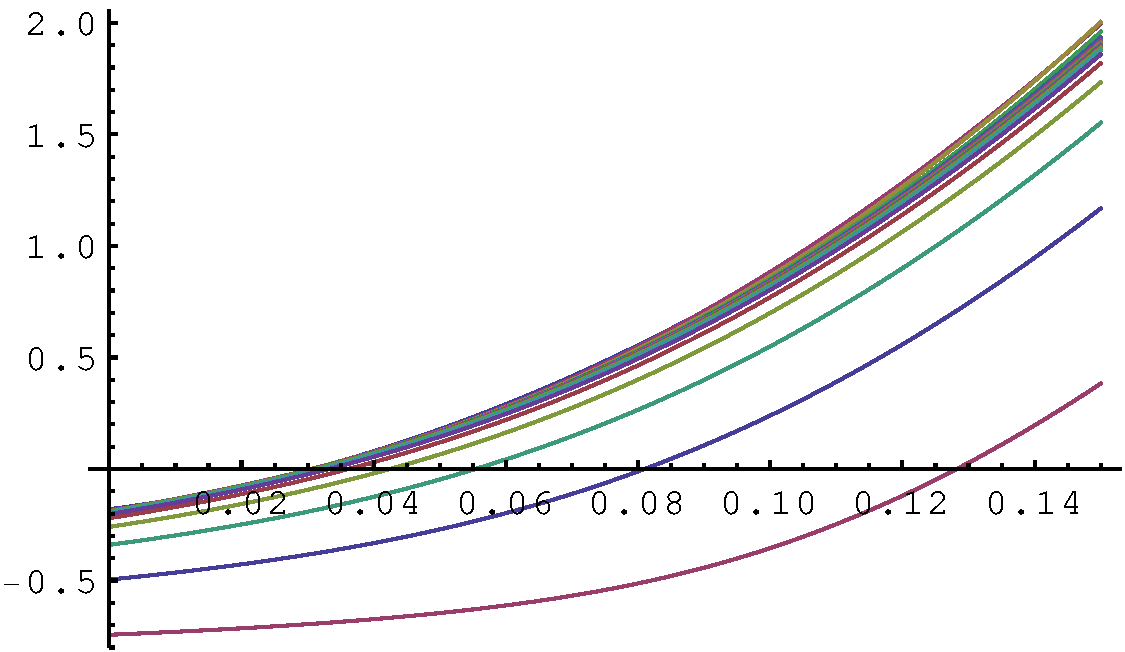
\includegraphics[scale=0.6]{img/chap4/u_flow_ising.pdf}
\caption{The potential for the Ising model at different times (local potential approximation was used). The accumulation of shapes tells us that we started close from a fixed point.}
\label{fig:u_flow_ising}
\end{center}
\end{figure}

An idea is to start from a shape for the potential at the microscopic scale, and plug it as an initial condition of the flow equation to see how the potential evolve in time. Here we took $u_{t=0}(\rho) = u_0 + \sigma \rho + u_4 \rho^2$ for the initial condition. We see that $\sigma$ is the temperature at the microscopic scale.
If at first the potential is almost stationary, that means we have started close from a critical point.
 By trial and error, \textit{i.e.} by fine-tuning of the temperature at microscopic scale, we can start closer and closer from the critical point. Once we have a sufficient precision, we can compute the critical exponents associated to this critical point. We tried this method with some success on the Ising model (fig. \eqref{fig:u_flow_ising}).
 
Several drawbacks entail this method. First, we have to solve a partial differential equation, which take some time. Secondly and more importantly, once we have found a critical point, it is hard to know which one it is if there exist several ones (which is the case for the Lifshitz model in $d = 3$).

For all this reasons, we used another approach: solving directly the fixed point equation, which is only a differential equation. This approach has, as we are going to see, the extra advantage of letting one locate with ease a fixed point of interest.

The equation we are interested in solving is 
\begin{equation}
0 = -d_m u(\rho) +(\theta \eta_\sslash + d_m - 4 \theta) \rho u'(\rho) + 8 v_m v_{d-m} \left( l_0^{dm}\left(u'(\rho) + 2 \rho u''(\rho) \right) + (n-1)l_0^{dm}\left(u'(\rho)\right) \right)
\end{equation}
Recalling that the $l_0$ functions are defined by an integral, we see that this is an implicit second order nonlinear differential equation, whose general solution is not known. One may wonder if there exists a clever choice of regulator that let us compute the integral, thus turning the nonlinear differential algebraic equation into a simple nonlinear differential equation. 
For the Ising model (in the local potential approximation), such a form of regulator is indeed known\footnote{It is the so-called $\theta$ regulator, $R_t(q)= (k^2-q^2) \theta\left(1-q^2/k^2\right)$}. For the Lifshitz model, it is not known if there exists a regulator allowing one to compute the integral explicitly. However we found a form of regulator allowing one to compute the integral approximately. Under this approximation -- which is explained and justified in appendix \ref{app:approx} -- the fixed point equation becomes
\begin{equation}
\label{eq:u_approx}
0 = u(\rho) - a(\theta, \eta)  \rho u'(\rho) + b_1(\theta, \eta) b_2(\theta, \eta, \rho_0) \left( \frac{1}{1 + \rho_0 + u'(\rho) + 2 \rho u''(\rho)} + \frac{n-1}{1+\rho_0+u'(\rho)} \right)
\end{equation}
This is an explicit second order nonlinear differential equation that depends on three parameters: $\eta$, $\theta$ and $\rho_0$. 
Of course the temperature also is a tunable parameter, appearing in the initial condition of the equation. Indeed, we have $u'(\rho=0) = \sigma$, the temperature. $u(0)$ is also linked to the temperature by $u(0) = n b_1 b_2/(1+\sigma)$.

By simply setting the value of the couple $(\sigma, \rho_0)$ we can place ourselves at any point of the two-dimensional phase diagram of the Lifshitz model.
Since this is the \textit{fixed point equation} for the potential, solving it returns the potential at the critical point $(\sigma, \rho_0)$. What happens when $(\sigma, \rho_0)$ is not a critical point? It turns out that the then unphysical solution of the fixed point equation blows up at some finite value of the field $\rho_{\text{sing}}(\sigma, \rho_0)$. 

This provides us with an easy way of finding fixed points. They correspond to points where the potential is defined for all values of the field, \textit{i.e.} to points such that $\rho_{\text{sing}}(\sigma, \rho_0)$ diverges. See fig. \eqref{fig:on_fp} for an illustration of this procedure in the simpler $O(n)$ case, which we tried before the Lifshitz case. 

\begin{figure}[htp]
\centering
\begin{subfigure}{.55\textwidth}
	\centering
	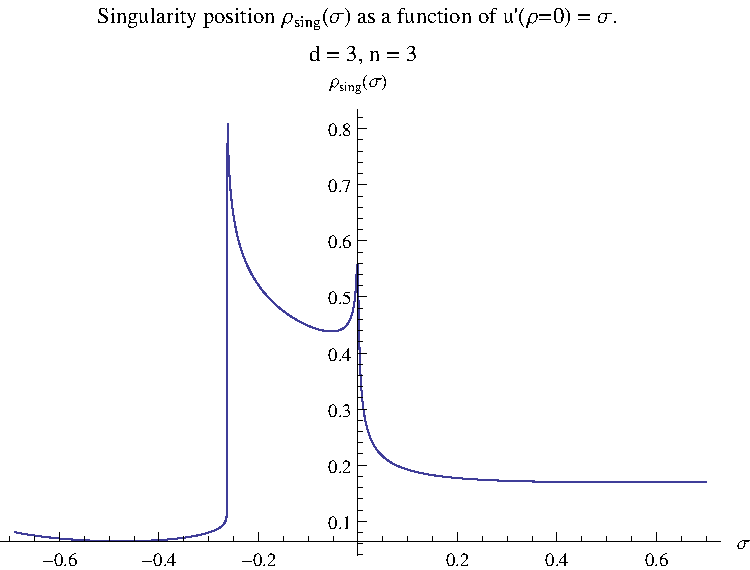
\includegraphics[width=.9\linewidth]{img/chap4/on_d3_n3.pdf}
	\caption{$d=3$}
	\label{on_d_3}
	\end{subfigure}%
\begin{subfigure}{.55\textwidth}
	\centering
	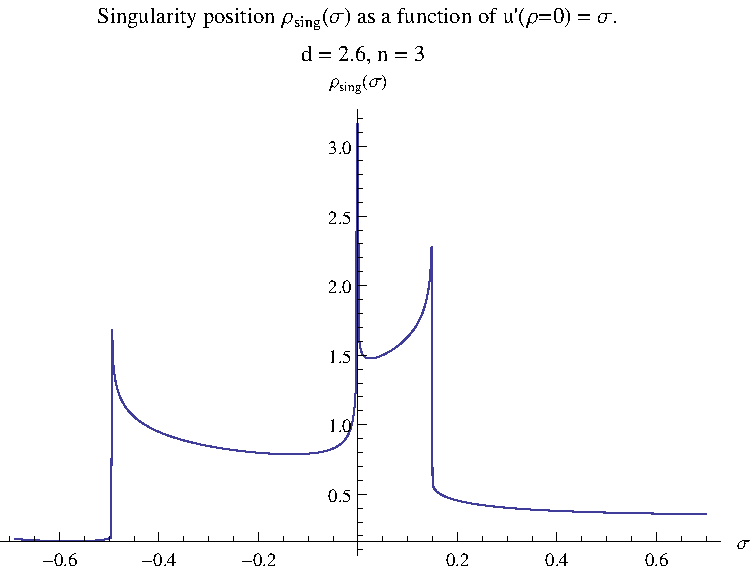
\includegraphics[width=.9\linewidth]{img/chap4/on_d2p6_n3.pdf}
	\caption{$d=2.6$}
	\label{on_d_2p6}
\end{subfigure}
\caption{Plot of the (numerically computed) explosion location $\rho_{\text{sing}}$ for the $O(n)$ model in the local potential approximation. We see that in $d=3$ only two physical solutions exist. They are the Gaussian fixed point, at $\sigma = 0$, and the Wilson-Fisher fixed point at its left. A second non trivial fixed point appears at $d = 8/3 \simeq 2.6$.}
\label{fig:on_fp}
\end{figure}

Once the critical temperature and $\rho_0$ are found, knowing the potential solution of the fixed point equation at this critical point we can compute the critical exponents. This method has already been applied successfully to the Ising \cite{CodelloIsing} and $O(n)$ \cite{CodelloOn} models. This was the first time it was tried on the Lifshitz model.
 The Lifshitz case is a slightly more complicated as it has two dimensional phase space, instead of a one dimensional one. This means that we must solve a system of two equations: the fixed point equation on the potential, and the fixed point equation on $\rho_0$, in order to fix the value of the two parameters.

We have not yet discussed the fate of the free parameters $\theta$, $\eta_\sslash$. In the local potential approximation, which we have considered here, they take their mean field value: $\theta \simeq \theta_{\text{mean field}} =  1/2$, $\eta_\sslash \simeq \eta_{\sslash\text{~mean field}} = 0$.
Beyond the mean field approximation, we must make use of the equations \eqref{eq:flow_perp}, \eqref{eq:flow_ss} to constrain the anomalous dimensions. We have derived these two equations, but had no time to go beyond mean field and use them.


To sum up, we have adopted the following strategy:
\begin{itemize}
\item Start at $d=d_c^>$, where mean field is exact in the sense that $\rho_0 = 0$.
\item Slightly decrease the dimension: $d \rightarrow d - \delta d$. 
\item Find the temperature of the Lifshitz point, by fine tuning of $\sigma$, using the fixed point equation on $u$ (eq. \eqref{eq:u_approx}).
\item Find how the value of $\rho_0$ has been modified by this shift in dimension and in temperature, using the fixed point equation on $\rho_0$ (eq. \eqref{eq:flow_rho}).
\item Go back to step two.
\end{itemize}
We have followed this algorithm until we reached $d=3$, at which point our results concerning critical exponents could be compared with the ones obtained by other means.

\subsection{Fixed point potential at the Lifshitz critical point}

\begin{figure}[htp]
\begin{center}
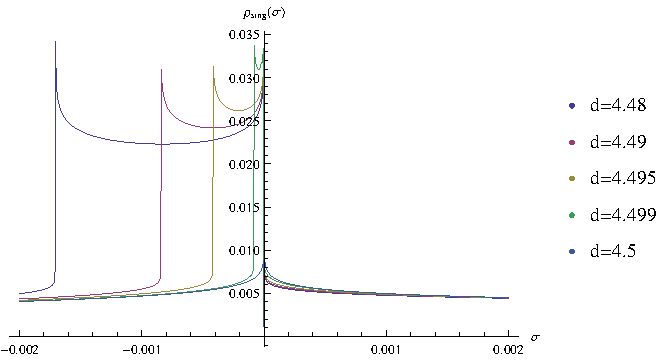
\includegraphics[scale=1]{img/chap4/emergence_lif.pdf}
\caption{Emergence of the Lifshitz fixed point (at the left of the $\sigma = 0$ Gaussian fixed point), when $d$ is slightly lowered, starting from $d_c^>$. Here we have chosen $m=1$ (and thus $d_c^> = 4.5$) and $n=3$.}
\label{fig:emergence_lif}
\end{center}
\end{figure}

\begin{figure}[htp]
\centering
\begin{subfigure}{.5\textwidth}
	\centering
	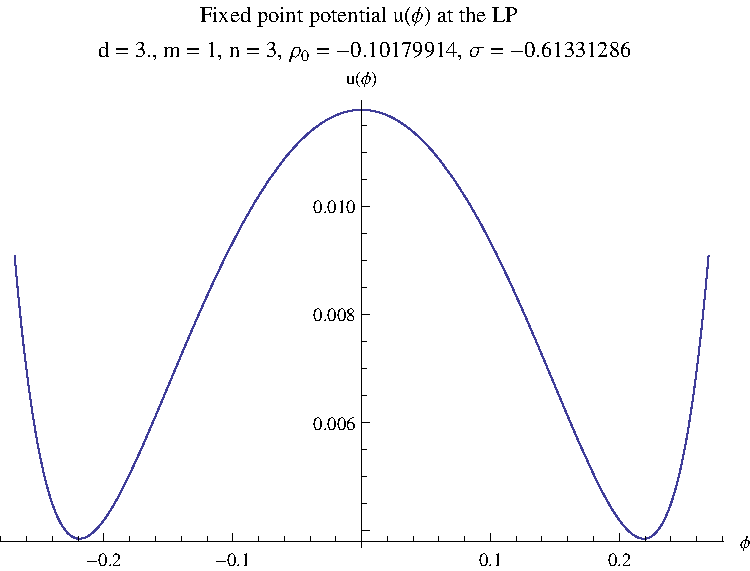
\includegraphics[width=.9\linewidth]{img/chap4/plotfieldd3.pdf}
	\caption{}
	\label{fig:plotfield}
	\end{subfigure}%
\begin{subfigure}{.5\textwidth}
	\centering
	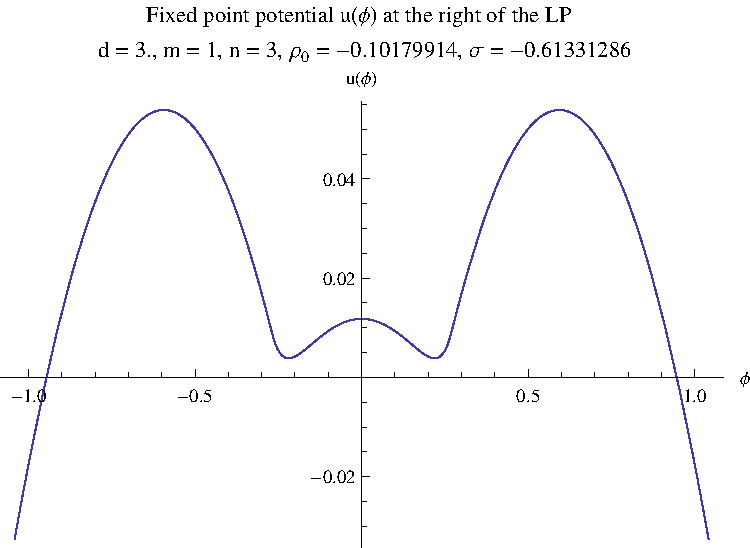
\includegraphics[width=.9\linewidth]{img/chap4/plotfieldrightd3.pdf}
	\caption{}
	\label{fig:plotfieldright}
\end{subfigure}
\caption{Shape of the potential at the Lifshitz point (left image) and and close to it (right image). $\phi$ is the module of the field (here tridimensional): $\phi \define \sqrt{\phi_i \phi_i}$.}
\label{fig:pot_d3}
\end{figure}

Figure \eqref{fig:emergence_lif} shows how the Lifshitz fixed point emerges at the left of the Gaussian fixed point, when $d$ is slowly lowered starting from $d_c^>$. It is remarkable that, in spite the approximation we made, the Lifshitz point appears precisely at $d = d_c^>$.

Figure \eqref{fig:plotfield} shows the shape of the dimensionless potential at the Lifshitz point. It has the standard ``Mexican-hat'' structure. Note that for an initial condition $\sigma$ very close to the Lifshitz point initial condition, the shape of the potential is completely different (fig. \eqref{fig:plotfieldright}). In particular it has the unphysical properties of going to $-\infty$ in the large field limit, meaning that it is not a confining potential. This high sensitivity to the variations of $\sigma$ in the neighborhood of the Lifshitz (or in fact any of any) fixed point allowed us to fine-tune the value of $\sigma_{\text{Lifshitz}}$ up to 12 decimal places very easily. This fine-tuning is essential in order to obtain accurate critical exponents.

\begin{figure}[htp]
\begin{center}
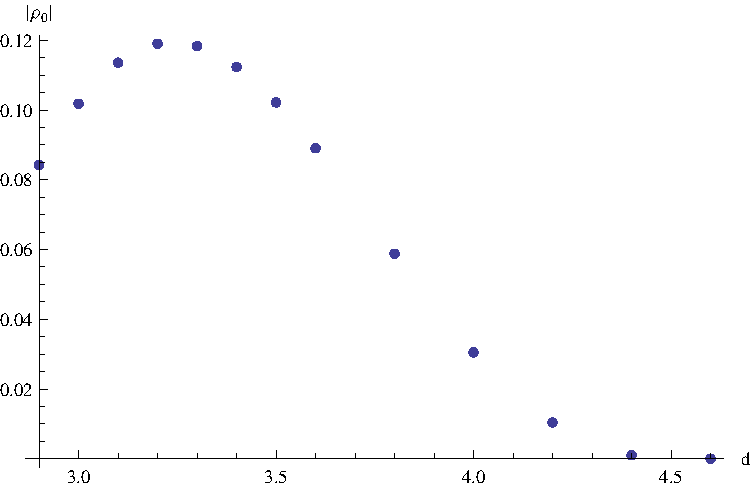
\includegraphics[scale=0.7]{img/chap4/rhod.pdf}
\caption{The parameter $\rho_0$ as a function of the space dimension $d$.}
\label{fig:rhod}
\end{center}
\end{figure}

To compute $\rho_0$, we make use of the its flow equation (eq. \eqref{eq:flow_rho}). At a fixed point, it simply is an algebraic equation on $\rho_0$, depending parametrically on the fixed point potential, which depends parametrically on $\rho_0$.  This means that formally we can write the problem as the self-consistent equation $\rho = f(\rho, u(\rho))$. To solve the problem we simply compute iteratively the sequence $\rho^{(n+1)} = f(\rho^{(n)}, u(\rho^{(n)}))$ until we reach a fixed point. By starting close to $d_c^>$ and progressively going down in dimension we thus obtain $\rho_0$ at the Lifshitz critical point as a function on $d$. The result is shown in fig. \eqref{fig:rhod}. 


Before we go on with the computation of the critical exponents, we will say a word on the numerical methods we used. For solving the nonlinear differential equation on the potential (eq. \eqref{eq:u_approx}), a simple Runge-Kutta method did not proved sufficiently accurate, because of the stiffness of the equation. Two methods were found well adapted to this stiff equation: Burlisch-Stoer's extrapolation scheme and the backward differentiation formula method. The latter proved the most accurate in our case. We therefore ended up using an order 5 BDF method to solve our fixed point equation.\footnote{The BDF implicitly express $u(\rho + \Delta \rho)$ in terms of $u(\rho)$, $u(\rho - \Delta \rho)$, $u(\rho - 2 \Delta \rho)$... At each ``time step'' $\Delta \rho$, this implicit equation must be solved to get $\rho + \Delta \rho$. We used Newton's method for that purpose.} 
To solve the algebraic equation on $\rho_0$ we simply used Newton's method.

\subsection{Critical exponents}

\begin{figure}[htp]
\centering
\begin{subfigure}{1.\textwidth}
	\centering
	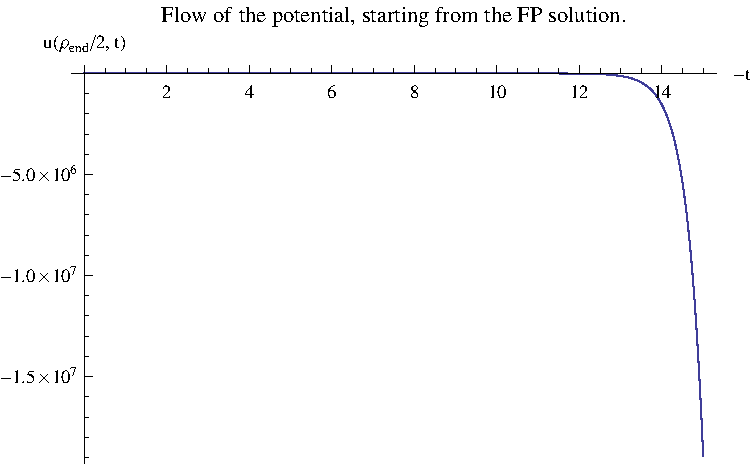
\includegraphics[width=.5\linewidth]{img/chap4/plotflowd3.pdf}
	\caption{Flow of the potential. Numerically, the potential is defined for $\rho \in [0, \rho_{\text{end}}]$ and here we chose arbitrarily to plot it at $\rho = \rho_{\text{end}}/2$.}
	\label{fig:plotflow}
	\end{subfigure}\\
\centering
\begin{subfigure}{.5\textwidth}
	\centering
	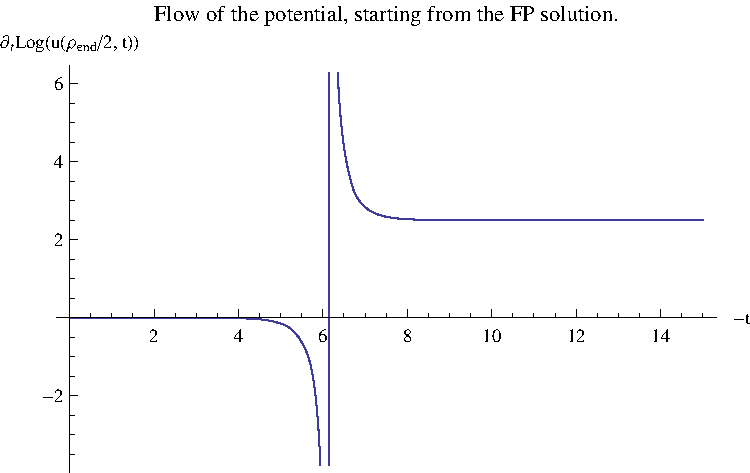
\includegraphics[width=.9\linewidth]{img/chap4/plotlogflowd3.pdf}
	\caption{$\p{t} \log{u_t}$ as a function of time.}
	\label{fig:plotlogflow}
	\end{subfigure}%
\begin{subfigure}{.5\textwidth}
	\centering
	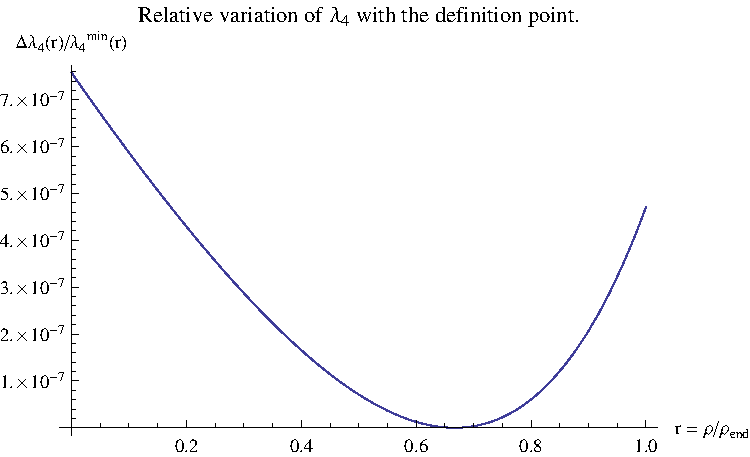
\includegraphics[width=.9\linewidth]{img/chap4/plotnud3.pdf}
	\caption{Relative variation of $\lambda_4$ with its definition point.}
	\label{fig:plotnu}
\end{subfigure}
\caption{}
\label{fig:flow}
\end{figure}

We recall that close to criticality the correlation length behaves as $\xi \propto |T - T_c|^{-\nu}$. 
In the case of the Lifshitz model, the existence of two nonequivalent directions implies the existence of two correlation lengths, and of two critical exponents traditionally denoted $\nu_4$ and $\nu_2$, corresponding to correlation lengths in the $\sslash$ and $\perp$ directions respectively. 

If we had numerically computed the fixed point potential $u(\rho)$ with infinite accuracy, then, when plugging it as an initial condition of the flow equation for the potential (eq. \eqref{eq:flow_u}), it should not evolve at all. That is to say, we should have $u_t(\rho) = u(\rho)$ for all $t$. 
Of course, we always have a finite accuracy on the fixed point potential, and when plugging it as an initial condition of the flow equation, the potential evolve in time, slowly going away from the critical surface. In the Lifshitz case two ``directions'' in the space of coupling constants are relevant ; one corresponding to $\nu_4$ and one corresponding to $\nu_2$. We thus have, 
\begin{equation}
u_t(\rho) = u(\rho) + \delta u_4(\rho) e^{\lambda_4 t} + \delta u_2(\rho) e^{\lambda_2 t}
\end{equation}
at the dominant order.
As we have seen, $\nu_4 = 1/\lambda_4$ and $\nu_2 = 1/\lambda_2$. Since $\nu_4 = \theta \nu_2 \leq \nu_2$, we have
\begin{equation}
u_t(\rho) \simeq u(\rho) + \delta u_4(\rho) e^{\lambda_4 t} 
\end{equation}
in the long time limit. That is to say, we should have $\p{t} \log{u_t(\rho)} \simeq \lambda_4$ when $t$ is sufficiently large. This is exactly what we obtain (fig. \eqref{fig:plotlogflow}).
This is how we measured $\lambda_4$ and thus $\nu_4$. 

We may wonder if these results depend on the point $\rho$ at which we compute $\p{t} \log{u_t(\rho)}$. We computed the relative variation of $\lambda_4$ with respect to the definition point (fig. \eqref{fig:plotnu}), to see that these variations only affect the sixth decimal place in the exponent. They are therefore completely negligible compared to other sources of errors.

The values of the critical exponents we found are in very good agreement with the perturbative expansion at order $\epsilon^2$ \cite{MouhannaLif}.
They also agree well with results obtained with another non-perturbative approach using the so-called Wilson-Polchinski equation \cite{BervillierLif}.  The results from this different approaches are compiled below.

\begin{center}
\label{tab:results}
\begin{tabular}{|c|c|c|c|}
\hline 
\rule[-1ex]{0pt}{2.5ex} ~ & our results & perturbative expansion & Wilson-Polchinski \\ 
\hline 
\rule[-1ex]{0pt}{2.5ex} $\nu_4$ & 0.399 & 0.392 & 0.317 \\ 
\hline 
\rule[-1ex]{0pt}{2.5ex} $\nu_2$ & 0.799 & 0.798 & 0.634 \\ 
\hline 
\end{tabular} 
\end{center}

So, apparently, the study conducted during this internship was only successful in finding the same results with a new method!
However, contrary to the Wilson-Polchinski approach, ours can be very easily extended to take into account the anomalous dimensions. In fact, computing the anomalous dimensions is as simple as computing $\rho_0$. All we have to do is use the fixed point (algebraic) equations on $\eta_\sslash$ and $\eta_\perp$ we have already derived, to find the values of the anomalous dimensions, in a fashion completely similar to what have been done concerning $\rho_0$. This has not been done during the internship simply because of a lack of time.

Taking the anomalous dimensions into account completely modifies the values of the critical exponents (cf. \cite{MouhannaLif}). So, they seem to play a crucial role in the physics of the Lifshitz model. 
In that respect, it is interesting to note that continuation of the work began during this internship should provide us with values of the anomalous dimensions, computed with unpreceeding precision.\footnote{The anomalous dimensions have already been computed within the nonperturbative framework, at order 12 in the field. Our method should give us more precise results as it takes into account all orders in the field.}


\section*{\huge{Conclusion}}

Before starting this internship, I thought of the renormalization group as a conceptually important object, yet nearly impossible to implement in practice except in a handful of cases. 
I was thus as surprised as pleased to discover in Wetterich equation a powerful and very systematic way of implementing the ideas of the renormalisation group. 
From a more practical point of view, I enjoyed doing both analytical computations -- mainly to derive the flow equations of the model, as well as numerical simulations.


Though the work I did during these eight weeks can by no means be considered as an exceedingly original contribution, it was satisfying for me to work -- with some modest success, on a new approach to the Lifshitz model. 
Indeed, during the internship we were able to retrieve the already known critical exponents of the model, with satisfying precision. The approach we opted for: namely, solving directly the fixed point equation, has not been much used yet. The easiness with which we were able to solve the fixed point equation is a good omen: this approach could very well be fruitful when applied to other models. In particular, it should be powerful to probe complicated phase diagrams in search of fixed point.


Concerning the Lifshitz model, there is of course still many things to do. 

First of all, we could get rid of the approximation we made, simply by using at the fixed point equation on the derivative of the potential, instead of solving the equation on the potential. Indeed, the equation on the derivative is an \textit{explicit} differential equation, while the equation on the potential is in general \textit{implicit}. Unfortunately, this idea occurred to us only at the end of the internship, and while we had enough time to test it successfully on the $O(n)$ model,  we lacked time to implement it in the case of the Lifshitz model.

Secondly, including the anomalous dimensions in the game would probably be very interesting, since as we have said, they likely play an important yet poorly understood role in the Lifshitz model.